\chapter{Frame}\label{frame}
I \textbf{sistemi di riferimento} o \textbf{frame} sono fondamentali per definire le coordinate della geometria che stiamo
disegnando. Un sistema di riferimento \`e costituito da un punto, l'\textbf{origine}, e da dei vettori (2 in 2D, 3 in 3D),
gli \textbf{assi}.

Un sistema di riferimento pu\`o esssere, a sua volta, definito all'interno di un altro sistema di riferimento. Chiameremo
quindi \textbf{frame canonico} il sistema di riferimento che ha l'origine alle coordinate $(0, 0, 0)$.

\section{Subframe}
Sia $o$ un punto rispetto al frame canonico e siano $u, v$ due vettori, posso definire il frame
\[ F = \{ o, u, v \} \]
Ora possiamo definire le coordinare di punto rispetto al frame $F$:
\[ p_F = (x_F, y_F) \]
Se volessi ricavare le coordinate rispetto al frame canonico posso usare la seguente formula:
\[ p = o + x_Fu + y_Fv \]
\textbf{NOTA}: l'intensit\`a dei vettori che compongono gli assi di $F$ determinano anche la distanza che per $F$ indica
l'unit\`a.

\begin{example}
	Prendiamo ad esempio il frame $F = \{ (1, 1), (2, 0), (0, 2) \}$ e posizioniamo un punto $P$ alle coordinate $(1, 1)$
	rispetto a $F$.
	\begin{center}
		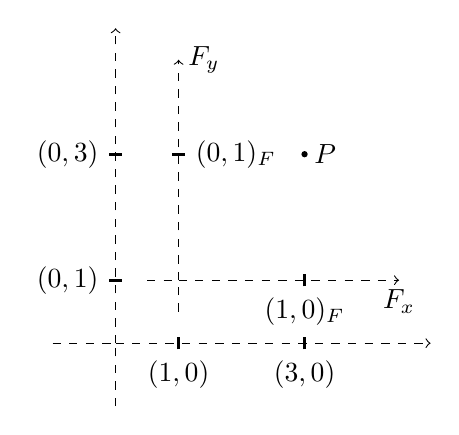
\begin{tikzpicture}[scale=0.8]
			% frame canonico
			\draw[dashed] (-1, 0) -- (0, 0);
			\draw[dashed] (0, -1) -- (0, 0);
			\draw[dashed, ->] (0, 0) -- (5, 0);
			\draw[dashed, ->] (0, 0) -- (0, 5);
			% riferimenti frame canonico
			\draw[very thick] (1, -0.1) node[below] {$(1, 0)$} -- (1, 0.1);
			\draw[very thick] (-0.1, 1) node[left] {$(0, 1)$} -- (0.1, 1);
			\draw[very thick] (3, -0.1) node[below] {$(3, 0)$} -- (3, 0.1);
			\draw[very thick] (-0.1, 3) node[left] {$(0, 3)$} -- (0.1, 3);
			% frame F
			\draw[dashed] (0.5, 1) -- (1, 1);
			\draw[dashed] (1, 0.5) -- (1, 1);
			\draw[dashed, ->] (1, 1) -- (4.5, 1) node[below] {$F_x$};
			\draw[dashed, ->] (1, 1) -- (1, 4.5) node[right] {$F_y$};
			% riferimenti F
			\draw[very thick] (3, 0.9) node[below] {$(1, 0)_F$} -- (3, 1.1);
			\draw[very thick] (0.9, 3) -- (1.1, 3) node[right] {$(0, 1)_F$};
			% punto
			\fill (3, 3) node[right] {$P$} circle [radius=0.05];
		\end{tikzpicture}
	\end{center}
	In generale \`e sbagliato pensare che le coordinate relative al frame canonico siano $(2, 2)$. Questo perch\'e il
	frame $F$ \`e composto da due vettori con intensit\`a 2. Svolgendo i calcoli infatti otteniamo:
	\[ p = (1, 1) + 1 (2, 0) + 1 (0, 2) = (3, 3) \]
	Che \`e ci\`o che abbiamo rappresentato in figura.

	Come possiamo notare, ci\`o che su $F$ equivale ad una distanza di un'unit\`a di misura	sull'asse $x$ per esempio,
	sul frame canonico equivale ad una distanza 2 unit\`a di misura. Questo perch\'e il vettore che definisce l'asse $x$
	di $F$ \`e $(2, 0)$.
\end{example}

In forma matriciale ho che la matrice
\[
	F = \begin{bmatrix}
		u_x & v_x & o_x \\
		u_y & v_y & o_y \\
		0   & 0   & 1
	\end{bmatrix}
\]
rappresenta il frame $F$ e se ho un punto $p$, espresso rispetto al frame $F$, e voglio ricavare le corrispondenti
coordinate rispetto al frame canonico mi basta fare questa operazione:
\[
	p = \begin{bmatrix}
		u_x & v_x & o_x \\
		u_y & v_y & o_y \\
		0   & 0   & 1
	\end{bmatrix}
	\begin{bmatrix}
		x_F \\ y_F \\ 1
	\end{bmatrix} =
	x_F \begin{bmatrix}
		u_x \\ u_y \\ 1
	\end{bmatrix} +
	y_F \begin{bmatrix}
		v_x \\ u_y \\ 1
	\end{bmatrix} +
	1 \begin{bmatrix}
		o_x \\ o_y \\ 1
	\end{bmatrix}
\]
Al contrario se ho le coordinate di $p$ rispetto al frame canonico e voglio ricavare le corrispondenti coordinate rispetto
a $F$ dovr\`o svolgere:
\[ p_F = F^{-1} p \]

\section{Passaggio tra frame non canonici}
Se ho due frame $F_1$ e $F_2$, entrambi non canonici, il passaggio di coordinate tra i due frame si effettua tenendo di
conto che
\[ p = F_1 p_1 = F_2 p_2 \]
dove $p$ indica un punto rispetto al frame canonico. Da qui ricaviamo facilmente la formula per il passaggio da un frame
all'altro, ad esempio da $F_1$ a $F_2$.
\[ p_2 = F_2^{-1} F_1 p_1 \]

\section{Trasformazione di frame}
In generale posso vedere un qualsiasi frame come il risultato della trasformazione di un altro frame.

Volendo posso anche trasformare un frame e muovere tutta la geometria con esso, in modo tale da avere le stesse coordinate
rispetto al frame iniziale.

Supponiamo di avere un punto definito rispetto al frame $F_1$, se io applicassi una matrice di trasformazione $A$ al punto
le coordinate rispetto a $F_1$ cambierebbero. Posso ottenere lo stesso effetto visivo applicando la matrice $A^{-1}$ al
frame. In questo modo $F_1$ si trasformer\`a in un altro frame $F_2$, il punto si trasformer\`a con esso ma le coordinate
del punto rispetto a $F_2$ saranno le stesse del punto rispetto a $F_1$.
\[ F_2 = A^{-1} F_1 \]

\section{Gerarchia dei frame}
\`E conveniente pensare ad una gerarchia dei frame in cui definisco una serie di frame rispetto ad altri frame, il tutto
per riuscire a definire piccole parti della scena in maniera pi\`u agevole e precisa, usando le coordinate vicino
all'origine degli assi. Molto pi\`u convieniente che utilizzare coordinate come (1000, 234, -242) per esempio.